\documentclass[12pt]{article}

\usepackage{amsmath}
\usepackage{mathtools}
\usepackage{tikz}
\usepackage{float}

\newtheorem{theorem}{Theorem}

\title{Double integrator with state and input constraints}
\author{Daniel Ricketts}

\newcommand{\vecbold}[1]{\boldsymbol{#1}}
\newcommand{\umin}{u_{min}}
\newcommand{\p}{\gamma}
\newcommand{\q}{\alpha}
\newcommand{\drawle}{-- (rel axis cs:1,1) -- (rel axis cs:1,0) -- (rel axis cs:0,0) \closedcycle}

\begin{document}
\maketitle

\section{Problem}
Consider the following double integrator:
\begin{align}
\begin{split}
\dot{x} &= v \\
\dot{v} &= u
\end{split}
\label{sys1}
\end{align}

We want constraints on $u$ so that this system satisfies the state
constraint $x \leq 0$ while obeying the input constraint $u \geq \umin$
where $\umin < 0$, under some assumptions on the initial state.

The formal details of a solution are below. Informally, the idea is that if
the pilot demands infinite positive acceleration, the system behaves as our
critically or over-damped linear system near the origin while issuing
constant acceleration $\umin$ farther away from the origin. Constant
acceleration implies a square root relationship between position and
velocity while the damped linear system implies a linear relationship. The
key to satisfying the above intuition is to form an invariant that is
linear near the origin and a square root farther away while having a smooth
transition between the two. This is done by shifting the square root curve
left until it is tangent to the linear constraint, as depicted in
Figure~\ref{fig:sqrt-lin}. The shaded region in Figure~\ref{fig:sqrt-lin}
depicts the invariant we would like to enforce. The step from the invariant
in Figure~\ref{fig:sqrt-lin} to $x \leq 0$ is relatively simple.

\begin{figure}[H]
\centering
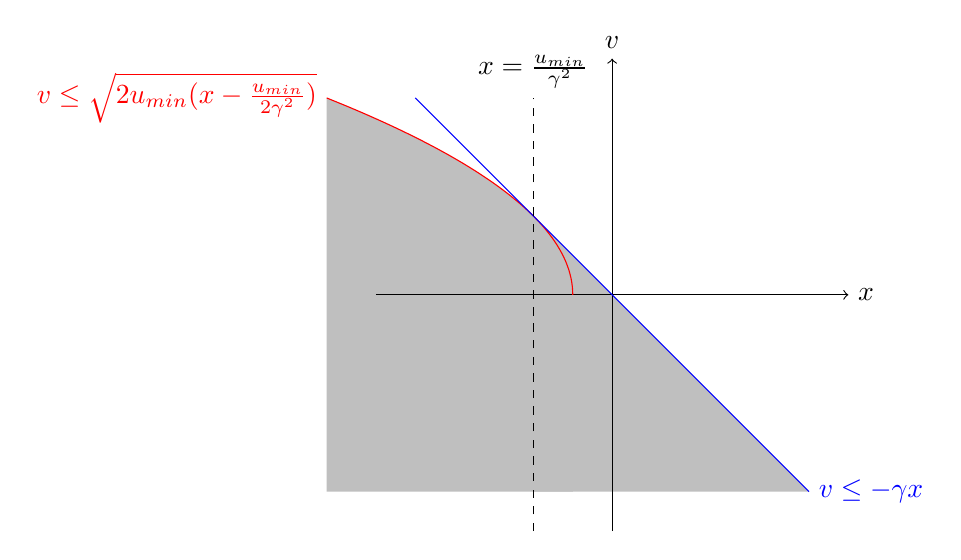
\begin{tikzpicture}
      \fill [lightgray, domain=0:2.5, variable=\x]
        (-0.5,-2.5)
        -- plot ({-\x*\x/2 - 1/2}, {\x})
        -- (-3.625, -2.5)
        -- cycle;
      \fill [lightgray, domain=-1:2.5, variable=\x]
        (-1, -2.5)
        -- plot ({\x}, {-\x})
        -- cycle;
      \draw[->] (-3,0) -- (3,0) node[right] {$x$};
      \draw[->] (0,-3) -- (0,3) node[above] {$v$};
      \draw[domain=0:2.5,smooth,variable=\v,red]  plot ({-\v*\v/2 - 1/2},{\v})
          node[left] at (-3.625,2.5) {$v \leq \sqrt{2\umin(x - \frac{\umin}{2\p^2})}$};
      \draw[domain=-2.5:2.5,smooth,variable=\x,blue]  plot ({\x},{-\x}) node[right] at (2.5,-2.5) {$v\leq -\p x$};
      \draw[black,variable=\x,domain=-3:2.5,dashed] plot ({-1},{\x}) node[above] at (-1,2.5) {$x = \frac{\umin}{\p^2}$};
\end{tikzpicture}
\caption{A depiction of $B(x,v) \leq 0$ where the red curve represents the first branch of the piecewise function and blue the second.}
\label{fig:sqrt-lin}
\end{figure}

Formally, the invariant is $B(x,v) \leq 0$, where
\[B(x,v) =
\begin{cases}
v - \sqrt{2\umin(x - \frac{\umin}{2\p^2})} & \text{if } x < \frac{\umin}{\p^2}\\
v + \p x & \text{otherwise}
\end{cases}
\]
for some constant $\p > 0$.

This induces the following constraints on $u$:
\[
u \leq
\begin{cases}
-\q(v - \sqrt{2\umin(-x + \frac{\umin}{2\p^2})}) - \frac{\umin v}{\sqrt{2\umin(-x + \frac{\umin}{2\p^2})}} & \text{if } x < \frac{\umin}{\p^2}\\
-(\q + \p) v -\q\p x & \text{otherwise}
\end{cases}
\]

In Section~\ref{sec:proof}, we will prove that this system satisfies the
state constraint $x \leq 0$ while obeying the input constraint $u \geq
\umin$ where $\umin < 0$, under the assumption that $x \leq 0$ and $B(x,v)
\leq 0$ hold on the initial state.

\section{Proof}
\label{sec:proof}
This proof proceeds in three steps:
\begin{enumerate}
\item Use the barrier function theorem to show that $B(x,v) \leq 0$ is an invariant of the system.
\item Use the above invariant and another application of the barrier function theorem to show that $x \leq 0$ is an invariant of the system.
\item Show that, within the invariant region, $u \geq \umin$.
\end{enumerate}

\paragraph*{Step 1}
The Lie derivative of $B(x,v)$ is as follows:
\[\dot{B}(x,v) =
\begin{cases}
u - \frac{\umin v}{\sqrt{2\umin(x - \frac{\umin}{2\p^2})}} & \text{if } x < \frac{\umin}{\p^2}\\
u + \p v & \text{otherwise}
\end{cases}
\]

Applying the exponential barrier certificate theorem results in the following constraints on $u$:
\[
u \leq
\begin{cases}
-\q\left(v - \sqrt{2\umin(x - \frac{\umin}{2\p^2})}\right) + \frac{\umin v}{\sqrt{2\umin(-x + \frac{\umin}{2\p^2})}} & \text{if } x < \frac{\umin}{\p^2}\\
-(\q + \p) v -\q\p x & \text{otherwise}
\end{cases}
\]

We have division by a variable in the first branch of the piecewise function, but due to
the condition on that branch ($x < \frac{\umin}{\p^2}$), the denominator is
at least $\frac{|\umin|}{\p} > 0$, so that term is bounded.

\paragraph*{Step 2}
We apply the barrier function theorem with a barrier function $x$, which
results in the constraint $v \leq -\p x$. Some algebra shows that $v + \p x
\leq B(x,v)$, which is easy to see from Figure~\ref{fig:sqrt-lin}. Since
$B(x,v) \leq 0$, we know that $v + \p x \leq 0$.

\paragraph*{Step 3}
We need to show that both branches of the piecewise constraint on $u$ are
at least $\umin$. For the first branch, since $\umin < 0$ and $B(x,v) \leq 0$, we know that
\[\frac{\umin v}{\sqrt{2\umin(-x + \frac{\umin}{2\p^2})}} \geq \umin\]
and
\[-\q\left(v - \sqrt{2\umin(x - \frac{\umin}{2\p^2})}\right) \geq 0\]
so the entire branch is at least $\umin$.

For the second branch, since $v \leq -\p x$,
\[-(\q + \p) v -\q\p x \geq (\q + \p - \q\p)x\]
If $\q+\p-\q\p < 0$, then since $x \leq 0$, $(\q+\p -\q\p)x \geq 0 >
\umin$. Otherwise, since $x \geq \frac{\umin}{\p^2}$, $(\q+\p -\q\p)x \geq
\umin$ as long as $\q + \p -\q\p \leq \p^2$.

\section{Exponential barrier functions}
The proof uses a general theorem about barrier functions. A barrier
function is a scalar function along trajectories of the system that is used
to establish an invariant. This particular flavor of barrier functions
establishes invariants of the form $B(\vecbold{x}) \leq 0$ where $B$ is the
barrier function. The theorem states that such a predicate is an invariant
of the system if the value of $B$ along trajectories of the system
approaches the boundary of the invariant no faster than an
exponential. More precisely:

\begin{theorem}
For an $n$-dimensional system, if there exists a function $B \in \mathcal{R}^n \rightarrow \mathcal{R}$ and some constant $\lambda \in \mathcal{R}$ such that
\[\dot{B}(\vecbold{x}) \leq \lambda B(\vecbold{x})\]
then the set $\{\vecbold{x} \in \mathcal{R}^n : B(\vecbold{x}) \leq 0\}$ is forward invariant. In other words, along all trajectories of the system $\vecbold{x}(t)$, if $B(\vecbold{x}(0)) \leq 0$, then $\forall t \geq 0, B(\vecbold{x}(t)) \leq 0$.
\label{thm:exp-barrier}
\end{theorem}

In this theorem, $\dot{B}(\vecbold{x})$ is the derivative of $B$ with
respect to time along trajectories of the system, also known as the Lie
derivative.

\end{document}
